\section{An\'alisis}

\subsection{Mediciones realizadas}
Se utilizaron tres ``trazas'' de sequencias de llamados (\textit{request} y \textit{release}):   
\begin{itemize}
\item \textbf{BNLJ}: se trata de una traza que simula el comportamiento de un algoritmo BNLJ para evaluar un join. 
El outer join consta de 400 p\'aginas, mientras que el inner join comprende 500 p\'aginas. 
Entre los tipos de traza \textit{puros} propuestos en el enunciado, este fu\'e el \'unico considerado individualmente, 
ya que vuelve a referenciar las mismas p\'aginas m\'as de una vez y tiene un compartemiento mas complejo que 
el ``Index Scan Uncluestered''. 
\item \textbf{Concatenado Aleatorio ``Peque\~no''}: se trata de una traza compuesta por una concatenaci\'on secuencial de 
las trazas b\'asicas del enunciado: \textit{File Scan}, \textit{Index Scan Clustered}, \textit{Index Scan Unclustered} 
y \textit{BNLJ}. Se generan 100 trazas aleatorias considerando instancias de estos cuatro tipos de trazas ``b\'asicos'',
siendo estas instancias relativamente pequeñas, generando una cantidad 900 pedidos en total, aproximadamente 9 por instancia). 
\item \textbf{Concatenado Aleatorio ``Grande''}: sigue el mismo esquema que el anterior pero sumando 1000 trazas b\'asicas y
generando unos 88.000 pedidos en total, aproximadamente 90 por instancia.
\end{itemize}

Cada estrategia considerada: Best, Random, MRU, LRU, FIFO y Count y para cada una de estas tres trazas propuestas se
midi\'o el \textit{hit rate} con distintos tama\~nos de de buffer. 

\subsubsection{Par\'ametros de la mediciones}
Para determinas los distintos tama\~nos de buffer se consideraron dos cotas que dependen de la traza y una decena de valores
intermedios entre ellos como se sugiere en \cite{eff84}. Ambas magnitudes (cota superior e inferior) son calculadas en la cĺase ``TraceUtil''
mencionada anteriormente.

\subsubsection*{Cota superior}
El tama\~no de buffer m\'aximo considerado para una determinada traza es la cantidad de p\'aginas distintas que se solicitan. Un buffer
de mayor capacidad que esta cantidad tendr\'ia siempre espacio libre.  

\subsubsection*{Cota inferior}
El tama\~no de buffer m\'inimo considerado para una determinada traza es la mayor cantidad de p\'aginas distintas que est\'an ``solicititadas''
en un determinado momento. Un buffer de menor tama\~no que esta cantidad no podr\'ia alamacenar todas las p\'aginas necesarias para la ejecuci\'on 
en el momento ``pico'' de solicitudes. Para calcular este n\'umero se simula la ejecuci\'on de una traza manteniendo la cantidad de p\'aginas abiertas
en cada operaci\'on y calculando el m\'aximo de todos estos valores. 

\subsubsection{Proceso de medici\'on}
La evaluaci\'on de las p\'aginas se encuentra implementada en la clase \textit{CompareStrategies} del paquete \textit{ubadb.bench}. 
Este proceso genera una salida con formato CSV. En los archivos adjuntos se presenta esta informaci\'on en una planillia de 
c\'alculo de tipo ODT para una lectura m\'as c\'omoda de los resultados y para posterior generaci\'on de gr\'aficos a partir de 
los mismos.

\subsection{Resultados}
A continuaci\'on se muestran los resultados de la eficiencia (\textit{hit rate}) en funci\'on del tama\~no del buffer, para cada una de las trazas usando cada una de las
estrategias.
\subsubsection*{Traza ``BNLJ''} 
\begin{center}
  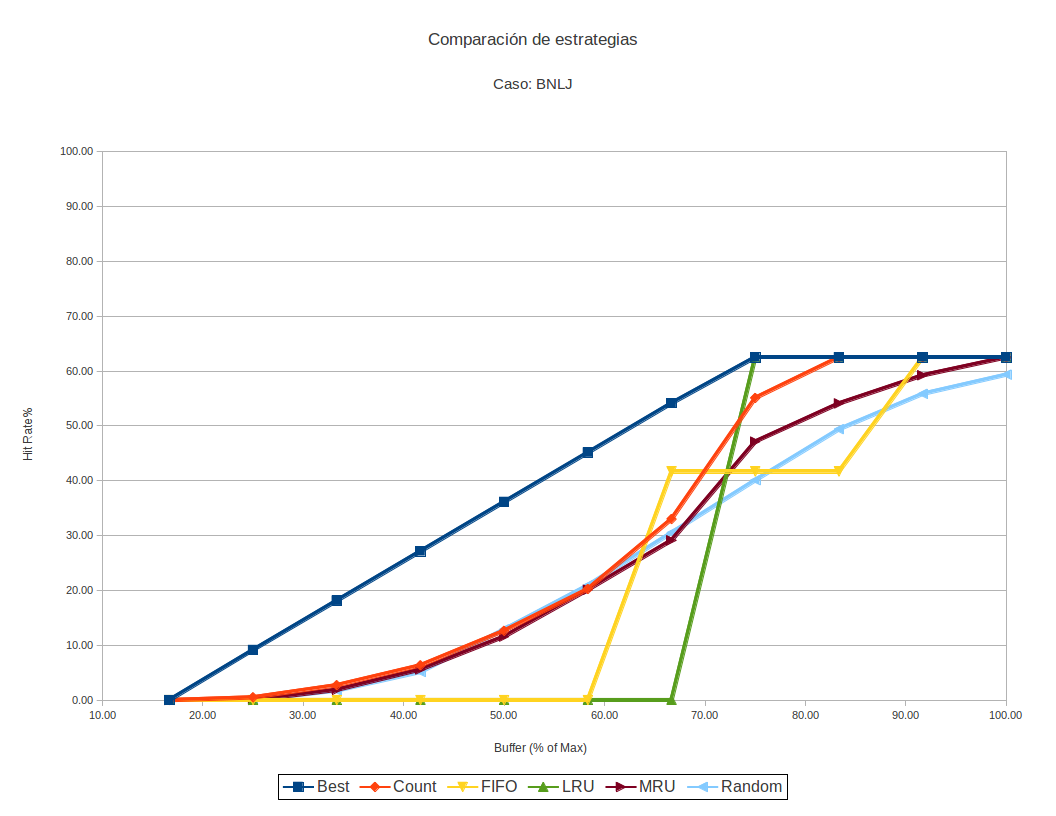
\includegraphics[height=11cm]{bnlj.png}
\end{center}  
\subsubsection*{Traza ``Peque\~na''} 
\begin{center}
  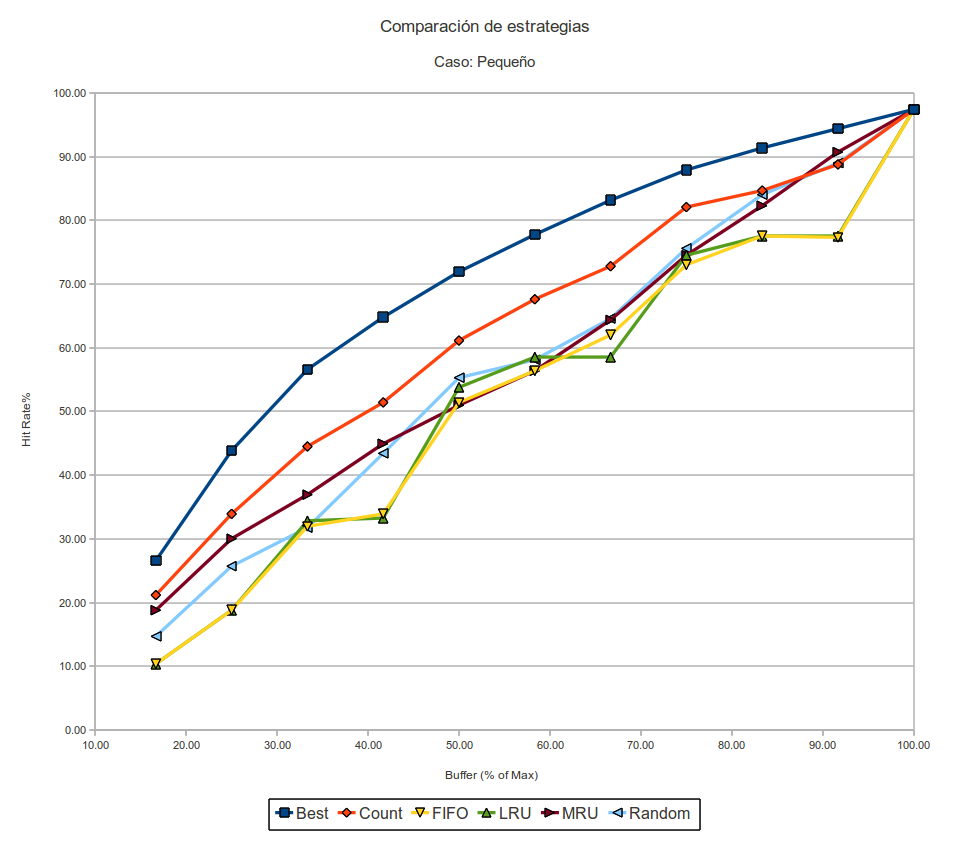
\includegraphics[height=11cm]{small.png}
\end{center}  
\subsubsection*{Traza ``Grande''} 
\begin{center}
  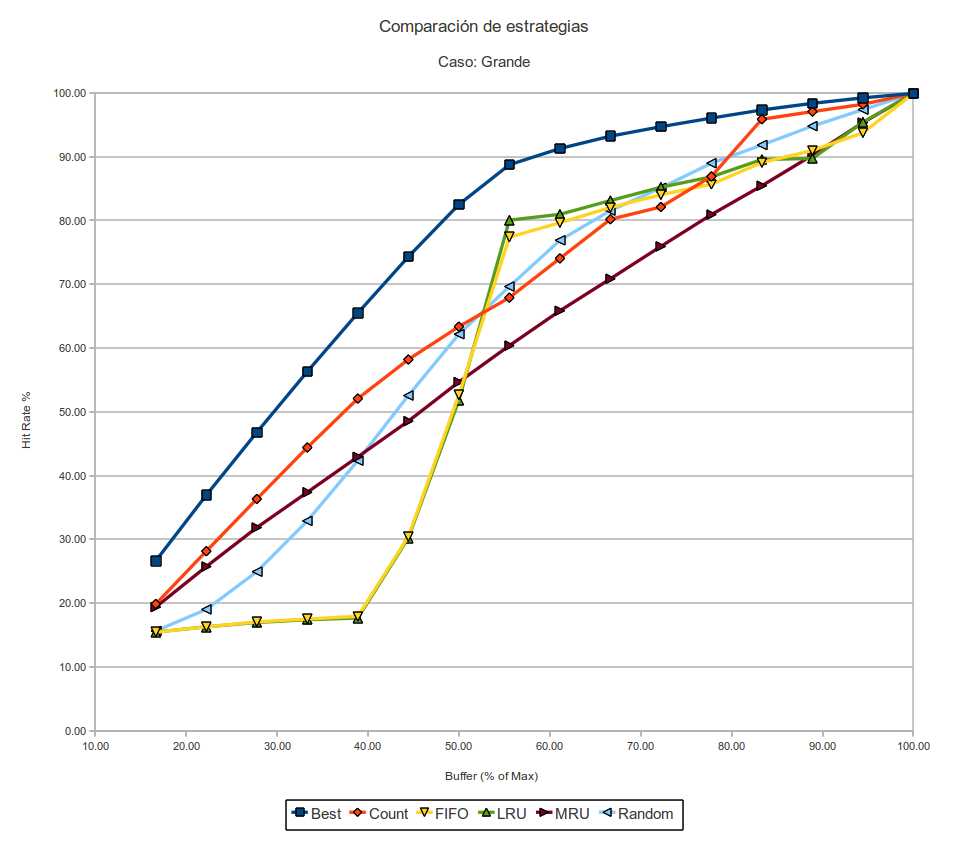
\includegraphics[height=11cm]{big.png}
\end{center}  


\subsection{An\'alisis de los resultados y conclusiones}

\subsubsection*{Traza ``BNLJ''}
En el caso de la traza de \textbf{BNLJ}, se ve que mientras tanto \textbf{MRU}, \textbf{Count} y \textbf{Random} mejoran su eficiencia conforme el tama\~no del buffer
va aumentando, a partir del $70\%$, \textbf{Count} supera a \textbf{MRU} y esta supera a \textbf{Random}. Por otra parte las estrategias \textbf{FIFO} y \textbf{LRU} tienen
mala respuesta de performance para buffers peque\~nos y buena respuesta para buffers de mayor capacidad. 

\subsubsection*{Traza ``Grande'' y ``Peque\~na''}
bla bla bla

\subsection{Tabla de comparaciones}
En funci\'on de los an\'alisis anteriores se presenta la siguiente tabla comparativa de eficiencia de las distintas estrategias en los distintos contextos:
\begin{center}
  \begin{tabular}{ | l | c | c | c | c | }
    \hline
    \multirow{2}{*}{Estrategia} & \multicolumn{2}{c|}{\textbf{BNLJ}} & \multicolumn{2}{c|}{\textbf{Aleatorio}} \\
    & Buffer Peque\~no & Buffer grande & Buffer Peque\~no & Buffer grande \\ \hline
    \textbf{Count} & Bueno & Bueno & Bueno & Bueno \\ \hline
    \textbf{MRU} & Bueno & Bueno & Bueno & Bueno \\ \hline
    \textbf{LRU} & Malo & Bueno & Malo & Bueno \\ \hline
    \textbf{FIFO} & Malo & Bueno & Malo & Bueno \\ \hline
  \end{tabular}
\end{center}